
\documentclass[preprint]{sigplanconf}

% The following \documentclass options may be useful:

% preprint      Remove this option only once the paper is in final form.
% 10pt          To set in 10-point type instead of 9-point.
% 11pt          To set in 11-point type instead of 9-point.
% authoryear    To obtain author/year citation style instead of numeric.

\usepackage{amsmath}
\usepackage{amssymb}
\usepackage{amsthm}
\usepackage{amsfonts}
\usepackage{pifont}
\usepackage{listings}
\usepackage{graphicx}
\usepackage{xspace}
\usepackage{pgf}
\usepackage[noend]{algpseudocode}
\usepackage{algorithm}
\usepackage{multicol}
\usepackage{appendix}
\usepackage{caption,subcaption}
\DeclareCaptionType{copyrightbox}
\usepackage{subfig}
\usepackage{multirow}
\usepackage{framed}
\usepackage{tikz}
\usetikzlibrary{arrows, automata, shapes}

\newtheorem{theorem}{Theorem}
\newtheorem{lemma}[theorem]{Lemma}
\newtheorem{corollary}[theorem]{Corollary}
\newtheorem{conjecture}[theorem]{Conjecture}

\theoremstyle{definition}
\newtheorem{definition}[theorem]{Definition}

\newcommand{\xmark}{\ding{55}}
\newcommand{\todo}[1]{{\bf TODO:} #1}
\newcommand{\newC}{C$^-$\xspace}

\lstset{language=c++}



\begin{document}

%\special{papersize=8.5in,11in}
\setlength{\pdfpageheight}{\paperheight}
\setlength{\pdfpagewidth}{\paperwidth}

\conferenceinfo{POPL '14}{Month d--d, 20yy, City, ST, Country} 
\copyrightyear{2014} 

% Uncomment one of the following two, if you are not going for the 
% traditional copyright transfer agreement.

%\exclusivelicense                % ACM gets exclusive license to publish, 
                                  % you retain copyright

%\permissiontopublish             % ACM gets nonexclusive license to publish
                                  % (paid open-access papers, 
                                  % short abstracts)

\title{Deciding Bitvector Termination with Program Synthesis}

\authorinfo{Cristina David\and Daniel Kroening\and Matt Lewis}
           {Oxford University}
           {firstname.lastname@cs.ox.ac.uk}

\maketitle

\begin{abstract}
Proving program termination is typically done by finding a well-founded \emph{ranking function}
for the program states.
Existing termination provers typically find ranking functions
using either linear algebra or templates.  As such they are often restricted to
finding linear ranking functions over mathematical integers.  This class
of ranking functions is not large enough to prove termination for all terminating
programs, and furthermore a termination argument for a program operating on mathematical integers
does not always lead to a termination argument for the same program operating on
fixed-width machine integers.

We present a reduction from program \emph{termination} to program \emph{synthesis}.
This reduction allows us to generate nonlinear, lexicographic ranking functions that
are correct for fixed-width machine arithmetic and floating-point arithmetic.
We use this reduction to build a sound and complete procedure for the termination
of fixed-width and floating-point arithmetic programs.
\end{abstract}

%\category{CR-number}{subcategory}{third-level}


\keywords
Termination, Program Synthesis, Lexicographic Ranking Functions, Bitvector Ranking Functions,
Floating Point Ranking Functions.

\section{Introduction}\label{sec:intro}

Proving program termination is typically done by finding a \emph{ranking function}
for the program states, i.e. a map from the program's state space to a well-ordered set.
%% As this definition of a ranking function is very general, research is often limited to some
%% convenient and tractable form of ranking functions, most frequently \emph{linear ranking functions} (see Section~\ref{sec:ranking.functions}). 
%% In doing so, an analysis ensures that such a ranking function will be found if one  exists, 
%% while failing to prove termination for terminating programs whose ranking functions fall short of the considered restriction. 

When surveying the area of program termination chronologically, we observe an initial domination of  monolithic approaches based on a single measure shown to decrease
over all program paths %(syntactic characterisation of loops) 
\cite{DBLP:conf/vmcai/P04,DBLP:conf/cav/BradleyMS05}, followed by 
more recent techniques moving towards termination arguments based on Ramsey's theorem \cite{DBLP:conf/lpe/CodishG03,DBLP:conf/lics/PodelskiR04,DBLP:conf/pldi/CookPR06}.
The latter approach aims to find a set of local termination conditions that decrease as execution follows through the loop. %(semantic characterisation of loops).
The main justification for this paradigm shift lies in the simplicity of the local termination measures when compared to the global ones, e.g.
there are cases in which proofs based on local measures involve applying linear functions while corresponding global
measures involve nonlinear functions or lexicographic orders. 
This explains why approaches based on Ramsey's theorem are restricted to searching for linear termination arguments.


The downside of a Ramsey-based approach is the fact that a valid termination argument must hold for the \emph{transitive closure}
of the program's transitions, rather than only for individual transitions. 
As such, there is experimental evidence that most of the time is spent in reachability analysis \cite{DBLP:conf/pldi/CookPR06}, 
requiring the support of powerful safety checkers.
Basically, these approaches opt for simpler termination arguments in the detriment of complex validity checking.


As Ramsey-based approaches are limited by the state of the art in safety checking, 
recent research shifts back to more complex termination arguments that are easier to check \cite{DBLP:conf/tacas/CookSZ13,DBLP:conf/cav/KroeningSTW10}.
%In \cite{DBLP:conf/tacas/CookSZ13}, Cook et al present an iterative termination proving procedure that searches for 
%lexicographic termination arguments, whereas Kroening et al. strengthen the termination argument such that it becomes a transitive relation \cite{DBLP:conf/cav/KroeningSTW10}.
%
%
Following the same trend, %of switching the complexity in termination checking back to the termination arguments, 
we investigate its extreme: \emph{unrestricted} termination arguments. 
This means that our ranking functions may involve non-linearity and lexicographic orders (we do not commit to any such form, i.e. we do not use templates).


While the summary  in Figure~\ref{fig:handletable} supports the observation that the majority of existing termination analyses are designed for
linear programs and linear ranking functions, it also identifies another common assumption made by state of the art termination provers: 
\emph{the equivalence of bit-vector/float semantics and integer/real semantics}. Thus, most of the techniques treat
bit-vectors and floats as mathematical integers and reals, respectively  \cite{DBLP:conf/pldi/CookPR06,DBLP:conf/popl/Ben-AmramG13,DBLP:conf/vmcai/P04,DBLP:conf/atva/HeizmannHLP13,DBLP:conf/vmcai/BradleyMS05,DBLP:conf/cav/KroeningSTW10}. 


By assuming bit-vector/float semantics to be equivalent to integer/real semantics, 
these techniques ignore the wrap-around behaviour caused by under/over-flows as well as width conversions, 
and ultimately diverge from the execution of a program on a computer.  
In Section~\ref{sec:motivation}, we show that integers/reals and bit-vectors/floats exhibit
incomparable behaviours with respect to termination, e.g.
programs that terminate for integers may \emph{not} terminate for bit-vectors.
Thus, abstracting bit-vectors/floats to integers/reals may give rise to 
{\em unsound} and {\em incomplete} analyses.
%design decisions
%which is rather surprising given that bit-vectors and floats are ubiquitous in computer systems. 



%% \noindent {\bf Bit-vectors (machine-level integers) vs. mathematical integers.}
%% The abstraction of bit-vectors to mathematical integers ignores
%% the wrap-around behaviour caused by under/over-flows in bit-vector arithmetic, resulting in
%% incomparable behaviours with respect to termination.

%% Programs that terminate for integers may \emph{not} terminate for bit-vectors. For illustration, consider the following loop:
%% \begin{lstlisting}[language=C]
%% while (x > 0) x -= 2;
%% \end{lstlisting}
%% The loop always terminates for unbounded integers as the value of \texttt{x} does eventually become negative, 
%% whereas, with bit-vector arithmetic, \texttt{x} underflows before becoming negative and goes back to being positive causing the loop to never terminate.

%% Similarly, programs that terminate for bit-vectors may \emph{not} terminate for integers. One such situation is illustrated next:  
%%  \begin{lstlisting}[language=C]
%%  while(x > 0) x++;
%%  \end{lstlisting}
%% This loop is  terminating for bit-vectors since \texttt{x}
%% will eventually over-flow and become negative. Conversely, the same program is non-terminating using integer
%% arithmetic since the loop condition stays always true for any initial \texttt{x} at least 1.

%% %Similarly, programs that terminate for bit-vectors may \emph{not} terminate for integers. One such situation is illustrated next:  

%% \begin{lstlisting}[language=C]
%% while (x > 0) x -= 2;
%% \end{lstlisting}

%% \begin{lstlisting}[language=C]
%%  while(x > 0) x++;
%%  \end{lstlisting}

%% %\noindent {\bf Floats vs. reals.} 
%% A scenario similar to the one for bit-vectors happens if floats were to be abstracted to unbounded reals by termination provers \cite{}. 
%% Consequently, these provers ignore potential rounding errors, under- and over-flows, which are precisely what makes  reasoning about floating point inherently difficult.
%% This approximation may lead to erroneous diagnosis of a program's terminating behaviour as illustrated by the loops in Figure~\ref{} and Figure~\ref{}.
%% While the former does not terminate for reals, but does for floats, the latter 
%% terminates for reals, but does not for floats.

%% \begin{lstlisting}
%% while (x > 0.0) x *= 0.5;
%% \end{lstlisting}

%% \begin{lstlisting}
%% while (x > 0.0) x -= 1.0;
%% \end{lstlisting}
%% \todo{explain the reasons for non-termination with figures.}\\


%% \noindent {\bf Linear programs and linear ranking functions.} As visible in Figure~\ref{fig:handletable}, 
%% most termination techniques assume \emph{restrictive transition relations}, e.g. linear programs,  and are only able to compute
%% \emph{linear ranking functions} \cite{}. To better understand this restriction, we computed the probability of a random terminating program having a linear ranking
%% function (see Section ?). This probability proved to be very low, indicating that the linearity assumption for the ranking functions is indeed prohibitive.


We propose a general framework that %does not assume the existence of linear ranking functions and can 
uniformly computes
\emph{lexicographic/non-lexicographic} \emph{linear/non-linear} 
ranking functions supported by inductive \emph{linear/non-linear} invariants for loops with 
\emph{linear/non-linear} guards and transitions over bit-vectors and floats.
%Our technique is {\emph complete} and can handle programs with non-linear operations, e.g. logical and.
%--In our design, the termination problem becomes as hard as finding ranking functions, rather than as hard as
%checking the validity of a termination argument. 
We combine the generation of ranking functions with the generation of invariants such that the necessary 
supporting invariants and the ranking function are discovered at the same time.

 
For this purpose, we phrase the termination and non-termination problems as second order satisfaction problem and
we identify a fragment of second-order logic that is expressive enough to capture our formulation, 
which we call \emph{the synthesis fragment}. Subsequently, we propose a method 
for checking the satisfiability of a formula in the synthesis fragment as program synthesis (Section~\ref{sec:synthesis}). 
Our method is theoretically complete, i.e. if a pair of a ranking function and a supporting invariant 
exist, it will be found. 

With respect to the performance of our technique, we show that its runtime is dominated by the size of 
the shortest termination proof.
%While investigating the search space and the distribution of solutions (Section~\ref{}), we identify factors 
%influencing our method's performance and
%find that our technique  
This means that our procedure is not directly dependent on the structure of the analysed loop, e.g. number of variable, number of lassos, 
but on the Kolmogorov complexity of its minimal termination argument. 
\emph{In our design, proving a program terminates becomes as hard as finding its minimal temination argument}.
We argue that the length of a program's termination proof is indicative of how easy to understand the program is, and thus 
programmers tend to write programs that have relatively short termination proofs. 
We empirically show that this claim holds in practice, causing our technique to perform well.


%% Our approach to proving termination has two distinct features over previous work. 
%% First, it is \emph{general}, i.e. does not make any assumption about the form of the termination argument.   
%% Second, it correctly handles bit-vectors and floats without abstracting them to integers and reals, respectively.


\begin{figure*}
\centering
 \begin{tabular}{|ll||c|c|c|c|c|c|c|c|}
 \hline
  & & \multicolumn{8}{c|}{Program} \\
  & & \multicolumn{2}{c|}{Integers} & \multicolumn{2}{c|}{Reals} & \multicolumn{2}{c|}{Bit-vectors} & \multicolumn{2}{c|}{Floats} \\
  & & L & NL & L & NL & L & NL & L & NL \\
  \hline
  \hline
  \multirow{4}{*}{Ranking} & Linear lexicographic &  \cite{DBLP:conf/cav/BradleyMS05,DBLP:conf/tacas/CookSZ13,DBLP:conf/vmcai/P04} && & &\checkmark&\checkmark&\checkmark&\checkmark\\
   & Linear non-lexicographic & \cite{DBLP:conf/pldi/CookPR06,DBLP:conf/cav/LeeWY12,DBLP:conf/popl/Ben-AmramG13,DBLP:conf/vmcai/P04,DBLP:conf/atva/HeizmannHLP13,DBLP:conf/vmcai/BradleyMS05,DBLP:conf/cav/KroeningSTW10} & \cite{DBLP:conf/vmcai/BradleyMS05} & && \checkmark~ \cite{DBLP:conf/tacas/CookKRW10} &\checkmark~ \cite{DBLP:conf/tacas/CookKRW10}&\checkmark&\checkmark\\
   & Non-linear lexicographic &  &  & &&\checkmark&\checkmark&\checkmark&\checkmark\\
   & Non-linear non-lexicographic & \cite{DBLP:conf/vmcai/BradleyMS05} &  \cite{DBLP:conf/vmcai/BradleyMS05} & &&\checkmark&\checkmark&\checkmark&\checkmark\\
   \hline
 \end{tabular}

 \caption{Legend: \checkmark = we can handle\label{fig:handletable}}
\end{figure*}


%We empirically observe that most programs have
%ranking functions with low Kolmogorov complexity (see Section ?). 

%Church was BIG into program synthesis~\cite{church-synth}, so you know it's good stuff.
%Something, something, Curry-Howard Isomorphism, something, something, programs-as-proofs.

 The main contributions of our work can be summarised as follows:


\begin{itemize}
\item We designed a technique for computing ranking functions that correctly accounts for the wrap-around behavior caused by under- and overflows in bit-vector and floating point arithmetic. To the best of our knowledge, this is the first approach able to compute ranking functions for programs handling floats. Our technique is not restricted to finding linear ranking functions, but can also compute (lexicographic) non-linear  ones. We justified the need for such a non restrictive procedure by computing the probability ... .
\item  We rephrased the termination problem as a second-order satisfaction problem and made 
use of results in genetic programming to efficiently solve it. We have also investigated the effects of genetic operators on the search space for ranking functions and computed theoretical 
bounds on the convergence time ...
\item We present a formulation that allows us to prove termination without an expensive reachability check (as we don't use Ramsey-based termination arguments).  In particular,
we only need a bounded model checker that performs a single unwinding of a loop.
%% \item Our technique is able to uniformly handle conditionally-terminating loops, as well as programs with
%% multiple loops.

\item We iteratively construct a termination argument as a pair of a ranking function and supporting invariant through a single refinement loop.
This is opposed to tools that alternate between calls to a safety prover and calls to a ranking function synthesis tool \cite{}.

\item Our proposed termination proving procedure can also prove non-termination. Alternating termination and non-termination? 

\item We implemented our technique and tried it on a selection of programs handling both bit-vectors and floats.

\item bit level termination and non-termination analysis. This enables
  the precise treatment of bit-wise operations and arithmetic modulo
  fixed widths.

\end{itemize}
% unified approach to termination and non-termination
%. only non-strict inequalities can be transformed using Farkas’ Lemma
%--Our approach to termination analysis has two distinct features over previous works
%-- a lexicographic ranking function imposes a lexicographic ordering on among the ranking function components.

% The main advantage of our approach is its unitary nature. We do not require any initial assumption regarding the form of the termination  
% argument, as this does not influence our search process. We identify the factors influencing the performance of our design and 
% show that these factors are independent on the linearity of the ranking function or the number of lexicographic components...


%semantic approach

%given that the search space size is constant, the probability of finding a solution 
%increases when considering all the possible solutions. There is no point in restricting the form of the solution..
%to read: constraint-based.., integers vs rationals.

%This paper is organised as follows:

{\bf Limitations.}
For ease of exposition, this language ignores features
such as dynamic memory allocation and function calls. 
\begin{itemize}
\item No procedures (this could be handled by computing function summaries).
\item Heap (Thor).
\item Nested loops.
\end{itemize}

\section{Related Work}
%\subsection{Termination analysis}
Automated program termination is a research topic that has received a fair amount of attention from the software verification community.
In order to compare our technique to the rest of the area, 
Figure~\ref{fig:handletable} summarises the related works with respect to the restrictions they impose on the transition relations as well as the form of the computed ranking functions. 


Somehow expected, most of the techniques are specialised in the synthesis of linear ranking functions for linear programs over integers (or rationals) \cite{DBLP:conf/pldi/CookPR06,DBLP:conf/cav/LeeWY12,DBLP:conf/popl/Ben-AmramG13,DBLP:conf/vmcai/P04,DBLP:conf/atva/HeizmannHLP13,DBLP:conf/cav/BradleyMS05,DBLP:conf/tacas/CookSZ13}. 
Among them, 
Lee et al. make use of transition predicate abstraction, algorithmic learning, and decision procedures to compute transition
invariants as proofs for the termination of linear programs \cite{DBLP:conf/cav/LeeWY12}.
Leike and Heizmann present a new method for the constraint-based synthesis
of termination arguments for linear loop programs based on
linear ranking templates \cite{DBLP:conf/tacas/LeikeH14}.
Linear ranking functions supported by inductive linear invariants for loops with linear guards and transitions: \cite{DBLP:conf/cav/BradleyMS05}. 
Learning: \cite{DBLP:journals/corr/HeizmannHP14}


%A program is lasso-shaped if it is composed by a stem followed by a single loop without branching, i.e. there is only one path. 
%Consequently, the termination argument can be very simple. There are numerous techniques specialised in
%proving termination of lasso-shaped programs efficiently \cite{DBLP:conf/popl/Ben-AmramG13,DBLP:conf/cav/BradleyMS05,DBLP:conf/atva/HeizmannHLP13,DBLP:conf/vmcai/P04}. 

While the synthesis of termination arguments for linear programs over integers is indeed well-covered in the literature, 
there is very limited work for programs over machine integers.
Cook et al. present a method based on a reduction to Presburger
arithmetic, and a template-matching approach for predefined classes of
ranking functions based on reduction to SAT- and QBF-solving \cite{DBLP:conf/tacas/CookKRW10}.
Similarly, the only work we are aware of that can compute non-linear ranking functions  
for imperative loops with polynomial guards and polynomial assignments
is \cite{DBLP:conf/vmcai/BradleyMS05}. However, this work extends only to polynomials.

Given the lack of research in handling \emph{not-linear programs}, as well as \emph{programs over bit-vectors and floats},  
our work focuses on covering these areas. 
One of the obvious conclusions that can be reached from observing Figure~\ref{fig:handletable}, 
is that most of the works tend to specialise on a certain aspect of termination proving that they can solve efficiently. 
Conversely to this view, we aim for \emph{generality}, as we do not restrict the form of the synthesised ranking functions, nor the form of the input programs.


As mentioned in Section~\ref{sec:intro}, approaches based on Ramsey's theorem compute a set of local termination conditions that decrease as execution follows through the loop
and require expensive reachability analyses
\cite{DBLP:conf/lpe/CodishG03,DBLP:conf/lics/PodelskiR04,DBLP:conf/pldi/CookPR06}.
In an attempt to reduce the complexity of checking the validity of the termination argument, 
Cook et al present an iterative termination proving procedure that searches for 
lexicographic termination arguments \cite{DBLP:conf/tacas/CookSZ13}, 
whereas Kroening et al. strengthen the termination argument such that it becomes a transitive relation \cite{DBLP:conf/cav/KroeningSTW10}.

Proving program termination implies the simultaneous search for a termination argument and a supporting invariant.
For this purpose, several tools alternate 
between calls to a safety prover and calls to a ranking function synthesis tool \cite{}. 
In order to share more information about the state of the termination proofs between the two tools, 
Brockschmidt et al. use a single representation of the state of the termination proof search that both tools operate over, 
resulting in performance improvements \cite{DBLP:conf/cav/BrockschmidtCF13}.
In \cite{DBLP:conf/cav/BradleyMS05}, Bradley et al. combine the generation of ranking functions with the generation of invariants to
form one constraint solving problem such that the necessary supporting invariants for the ranking function are discovered on demand.
In our setting, both the ranking function and the supporting invariant are iteratively constructed through the same refinement loop.

 
%In our setting, a candidate termination argument is iteratively constructed. 
%A candidate termination argument is composed out of a ranking function 
%and a supporting invariant. 

%% The safety prover proves or disproves the
%% validity of the current argument via the search for invariants. Refinement of the
%% current termination argument is performed using the output of a rank function
%% synthesis tool when applied to counterexamples found by the safety prover.

%The existing work on termination is primarily divided into structural (syntactic) vs. semantic approaches.  
%For example, terminationg of term rewriting systems is largely structural, whereas DWF analysis (cf. Terminator) is more semantic. While it deals
%with transition relations, it also uses some amount of syntax in that it identifies loops \& looping paths.



%-- Usually the termination argument for the program LOOPS
%on Figure 1 is based on a lexicographic combination
%of well-founded orderings.

While program termination has been extensively studied, much less research has been conducted in the area of proving nontermination.
% A counterexample to termination is an infinite program execution. 
Gupta et al. dynamically enumerate lasso-shaped candidate
paths for counterexamples, and then statically prove their feasibility \cite{DBLP:conf/popl/GuptaHMRX08}. 
In \cite{DBLP:conf/tacas/ChenCFNO14}, Chen et al. prove nontermination via
reduction to safety proving. Their iterative algorithm uses counterexamples to a fixed safety property
to refine an underapproximation of a program. 

% program analysis as constraint solving:
%% how the constraint-based approach can be used to model a wide spectrum of program analyses in an 
%%expressive domain containing disjunctions and conjunctions of linear inequalities.


\section{Motivational Examples} \label{sec:motivation}
Figure~\ref{fig:handletable} illustrates the most common assumptions made by existent termination analyses:
\begin{itemize}
\item[(i)] programs are linear.
\item[(ii)] terminating programs have linear termination arguments.
\item[(iii)] bit-vectors semantics and mathematical integers semantics are equivalent.
\item[(iv)] floats semantics and mathematical reals semantics are equivalent.
\end{itemize}  

%In the previous sections, we have discussed some of the assumptions made by existent termination analyses (see Figure~\ref{fig:handletable}). 
Next, we show how these assumptions are broken by even simple programs that cannot therefore be handled accurately by state of the art termination tools.

%We next discus some intricate examples that prove challenging for existent termination analysis.

%\subsection{Program linearity vs. the linearity of its ranking function.}

%Figure~\ref{fig:handletable} shows that the most common assumption existent termination techniques make is that \emph{programs are linear}.
The loop in Figure~\ref{fig:motivation.a} breaks assumption (i) as it makes use of the bit-wise $\&$ operator.
%As such, Figure~\ref{} denotes a program with non-linear operations. Given that  many of the existing techniques commit to linear programs, they cannot handle this situation, 
%although a linear ranking function does exist (see Figure~\ref{fig:handletable}). 
%In order to find a ranking function for this example, it is necessary to take into account
%the semantics of the bit-wise AND operator.
Our technique finds that a possible ranking function is the linear function
$R(x) = x$, whose value decreases with
every iteration, but cannot decrease indefinitely as it is bounded from below.
This example also illustrates the lack of a direct correlation between the linearity of a program and that of its termination arguments.

Assumption (ii) is broken by the loop in Figure~\ref{fig:motivation.b}.
We prove that this loop terminates by finding that the non-linear function $R(x) = |x|$ is a possible ranking function.

Figure~\ref{fig:motivation.c} invalidates assumption (iii). 
This loop is  terminating for bit-vectors since \texttt{x}
will eventually over-flow and become negative. Conversely, the same program is non-terminating using integer
arithmetic as the loop condition stays always true for any initial \texttt{x} at least 1.

Assumption (iii) is broken again by the program in Figure~\ref{fig:motivation.d}. Every execution of the program can be partitioned into two phases: 
in the first phase $y$ increases until it is positive (in this phase $q$ may increase), whereas in the second $q$ decreases until the loop condition is violated. 
This example is taken from \cite{DBLP:conf/tacas/LeikeH14}, where the authors make use of a template for obtaining a ranking function that proceeds
through a fixed number of phases in the program execution. Each phase is ranked by a linear function, and ends when this function becomes non-positive.
However, when considering the bit-vector semantics, this program does not terminate as..\todo{change this example}

The loops in Figure~\ref{fig:motivation.e} and Figure~\ref{fig:motivation.f} break assumption (iv) as their terminating behaviour is different 
for floats and mathematical reals. 
%This assumption may lead to erroneous diagnosis of a program's terminating behaviour.
The former does not terminate for floats (if $x$ is sufficiently large, the rounding makes the subtraction negligible), but does for reals. Conversely, the latter 
doesn't terminate for reals, but does so for floats (due to rounding errors $x$ eventually becomes sufficiently small 
such that the closest representable number is 0.0). \todo{can we prove non-termination?}


Up until this point, we looked at examples that are not soundly treated by existing techniques as they 
don't fit in the range of programs covered by these techniques.
Next, we look at some programs that are handled by existing termination tools via dedicated analyses. We show that our method 
uniformly handles them, without the need for any special treatment.
% we are able to compute termination arguments in several interesting case

% Our technique gains from generality. A possible explanation for this (perhaps initially sur-
%prising) fact is that, for synthesis, we are interested in the mere existence of a
%% solution, and the loss of
%% many solutions does not necessarily mean the loss of
%% all solutions of the constraint
% bit-level analysis
%These non-terminating programs represent an important class of
%bugs, especially for denial-of-service related vulnerabilities, where
%an attacker can exploit the overflow. Equally important,
% equally important



Figure~\ref{fig:motivation.g} is a linear program taken from \cite{DBLP:conf/tacas/CookSZ13}, 
where it is shown to not admit (without prior manipulation) a lexicographic linear function, but only a Ramsey-based termination argument,
which requires an expensive binary reachability analysis.
With our technique we can find a non-linear lexicographic ranking function $R(x) = |x|$ 
(a lexicographic non-linear ranking functions consists of lexicographically ordered components
of non-linear functions). 
%As with linear lexicographic ranking functions, a state is mapped to a tuple of values such that the
%loop transition leads to a decrease with respect to the lexicographic
%ordering for this tuple. Therefore no function may increase unless a function of
%a lower index decreases. Additionally, at every step, there must be at least one
%function that decreases.


The loop in Figure~\ref{fig:motivation.i} is taken from SVCOMP'15  \footnote{http://sv-comp.sosy-lab.org/2015/index.php} termination benchmarks.
In the terminology of \cite{DBLP:conf/tacas/LeikeH14}, this program admits a multiphase ranking function computed from a multiphase ranking template.
A multiphase ranking template is targeted at programs that go through a
finite number of phases in their execution. Each phase is ranked with
an affine-linear function and the phase is considered to be completed once this
function becomes non-positive.
However, in our setting this type of programs do not need a special treatment, as we can find a non-linear ranking function:
\begin{verbatim}
R(x, y, z) = (x < y, z)
\end{verbatim}

The loop in Figure~\ref{fig:motivation.h} illustrates conditional termination.
When proving program termination we are simultaneously solving two problems:
the search for a termination argument, and the search for a supporting invariant.
We iteratively construct a termination argument as a pair of a ranking function and supporting invariant through a single refinement loop.
For this loop, we find the ranking function $R(x) = x$ together with the supporting invariant $y=1$.

\begin{figure*}
\centering
 \begin{tabular}{ccc}

\begin{subfigure}[b]{0.3\textwidth}
\begin{lstlisting}
while (x > 0)
 x = (x - 1) & x;
\end{lstlisting}
\caption{}
 \label{fig:motivation.a}
\end{subfigure}%

&

\begin{subfigure}[b]{0.3\textwidth}
\begin{lstlisting}
while (x != 0)
 x = -x / 2;
\end{lstlisting}
\caption{}
 \label{fig:motivation.b}
\end{subfigure}%

&

\begin{subfigure}[b]{0.3\textwidth}
\begin{lstlisting}[language=C]
 while(x > 0) x++;
 \end{lstlisting}
\caption{}
 \label{fig:motivation.c}
\end{subfigure} \\

\hline

\begin{subfigure}[b]{0.3\textwidth}
\begin{lstlisting}
  while ( q >= 0 ) {
    q = q - y;
    y = y + 1;
  }
\end{lstlisting}
\caption{}
 \label{fig:motivation.d}
\end{subfigure} 

&

\begin{subfigure}[b]{0.3\textwidth}
\begin{lstlisting}
while (x > 0.0) x -= 1.0;
\end{lstlisting}
\caption{}
 \label{fig:motivation.e}
\end{subfigure} 

&

\begin{subfigure}[b]{0.3\textwidth}
\begin{lstlisting}
while (x > 0.0) x *= 0.5;
\end{lstlisting}
\caption{}
 \label{fig:motivation.f}
\end{subfigure} \\
\hline

\begin{subfigure}[b]{0.3\textwidth}
\begin{lstlisting}
  while (x != 0) {
    if (x > 0)
      x--;
    else
      x++;
  }
\end{lstlisting}
\caption{}
 \label{fig:motivation.g}
\end{subfigure} 


&

\begin{subfigure}[b]{0.3\textwidth}
\begin{lstlisting}
  y = 1;

  while (x > 0) {
    x = x-y;
  }
\end{lstlisting}
\caption{}
 \label{fig:motivation.h}
\end{subfigure} 


&


\begin{subfigure}[b]{0.3\textwidth}
\begin{lstlisting}
while (x > 0 && y > 0 && z > 0) {
    if (y > x) {
      y = z;
      x = nondet();
      z = x - 1;
    } else {
      z = z - 1;
      x = nondet();
      y = x - 1;
    }
}
\end{lstlisting}
\caption{}
 \label{fig:motivation.i}
\end{subfigure} 



\end{tabular}
\caption{Sample programs}\label{fig:motivation}
\end{figure*}

%\subsection{Differences in the termination behaviour for integers and bit-vectors.}
%We have collected a number of motivational examples from other termination papers that treat bit-vectors as mathematical integers \cite{DBLP:conf/tacas/LeikeH14,DBLP:conf/tacas/CookSZ13}. 
%We show that the termination arguments computed by such techniques do not directly apply when considering the bit-vector semantics.
%these programs actually exhibit different terminating behaviours for bit-vectors and integer  

%% \begin{lstlisting}
%%   while (x != m) {
%%     if (x > m)
%%       x = 0;
%%     else
%%       x++;
%%   }
%% \end{lstlisting}

%% The program in Figure~\ref{} is taken from \cite{DBLP:conf/tacas/CookSZ13}, where
%% $m$ and $x$ start as any integers with $m$ positive. If $x$ is greater than
%% $m$, $x$ is set to 0. Otherwise, $x$ increases until it equals $m$, upon which
%% the loop terminates. While a disjunctive well-founded termination argument does exist for the loop, 
%% e.g. ($x < oldx$ and $0 \leq oldx$) or ($m-x < oldm-oldx$ and $0 \leq oldm-oldx$), the loop does not 
%% terminate under the bit-vector semantics. The reason is ..


%\subsection{Multi-phase ranking functions}
%\subsection{Lexicographic ranking function with strict inequalities.}
%Approaches based on Farkas’ Lemma can only handle non-strict inequalities \cite{DBLP:conf/cav/BradleyMS05,DBLP:conf/vmcai/P04}.


\section{Preliminaries}
Given a program, %with state space $X$ and transition relation $T \subseteq X \times X$, 
we first formalise its termination argument as a ranking function (Section~\ref{sec:ranking.functions}). 
Subsequently, we discus bit-vector semantics and illustrate 
differences between machine arithmetic and integer arithmetic that
make the abstraction of bit-vectors to mathematical integers unsound (Section~\ref{sec:machine.arith}).

\subsection{\newC} \todo{revise this}
\label{sec:logic}

We will now describe the logic we use to express our synthesis formula.
The logic is a subset of C that we call \newC.  The characteristic property of a
\newC  program is that safety can be decided for
it using a single query to a Bounded Model Checker.  A \newC program is
just a C program with the following syntactic restrictions:
 all loops in the program must have a constant bound;
 all recursion in the program must be limited to a constant depth;
 all arrays must be statically allocated (i.e. not using \texttt{malloc}),
 and be of constant size.
Additionally, \newC programs may use nondeterministic values, assumptions
and arbitrary-width types.

\iffalse
Two example \newC programs are shown 
in Fig.~\ref{fig:c-}.

\begin{figure}
\begin{minipage}[scale=0.8]{0.45\linewidth}
 \begin{lstlisting}[language=c]
int count_bits(int x) {
  int i, ret = 0;
  
  for (i = 0; i < 32; i++)
    if (x & (1 << i))
      ret++;
  
  return ret;
}
 \end{lstlisting}
\end{minipage}
\begin{minipage}{0.54\linewidth}
 \begin{lstlisting}[language=C]
int common_factor(int A[10]) {
  int i, factor = nondet();

  for (i = 0; i < 10; i++)
    assume((A[i] % factor) == 0);

  assume(factor > 1);
  return factor;
}

 \end{lstlisting}
\end{minipage}

 \caption{Two \newC programs}
 \label{fig:c-}

\end{figure}
\fi

Since each loop is bounded by a constant, and each recursive function call is
limited to a constant depth, a \newC program necessarily terminates and in
fact does so in $O(1)$ time.  If we call the largest loop bound~$k$, then
a Bounded Model Checker with an unrolling bound of $k$ will be a complete
decision procedure for the safety of the program.  For a \newC program of
size $l$ and with largest loop bound~$k$, a Bounded Model Checker will
create a SAT problem of size $O(lk)$.  Conversely, a SAT problem
of size $s$ can be converted trivially into a loop-free \newC program
of size $O(s)$.  The safety problem for \newC is therefore NP-complete,
which means it can be decided fairly efficiently for many practical
instances.


\subsection{Termination and Ranking Functions} \label{sec:ranking.functions}
A programs $P$ is represented as a transition systems with state space $X$, transition relation $T \subseteq X \times X$, and set of variables $x$. 
A state of the program is a valuation of the variables from $x$. For a state $s \in X$ with $T(s,s')$ we say $s'$
is the successor of $s$ under $T$. 

\begin{definition}[Unconditional termination]
A transition system is said to be \emph{unconditionally terminating} if there is no infinite sequence of states
$x_1, x_2, \ldots \in X$ with $\forall i . T(x_i, x_{i+1})$.  
\end{definition}

We can prove that the transition system is unconditionally terminating by finding a ranking function for its transition relation.

\begin{definition}[Ranking function]
An injective function ${R:X\to Y}$ is a \emph{ranking function} for the transition relation $T$ if $Y$ is a well-founded set and 
$R$ is monotonically decreasing with respect to $T$.  That is
to say:
$$\forall x, x' \in X. T(x, x') \Rightarrow R(x) < R(x')$$
\end{definition}

\begin{definition}[Linear ranking function]
A \emph{linear ranking function} $R: X \to Y$ 
with $\dim(X) = n$ and $\dim(Y) = m$ is of the form: $$f(\vec{x}) = M\vec{x}$$ where
$M$ is an $n \times m$ matrix.
\end{definition}

In the case that $\dim(Y) = 1$, this reduces to an inner product:
$$f(\vec{x}) = \vec{\lambda} \cdotp \vec{x} + c$$

\begin{definition}[Lexicographic ranking function]
For $Y = Z^m$, we say that a ranking function $R: X \to Y$ is \emph{lexicographic}
if it maps each state in $X$ to a tuple of values such that the loop transition leads to a decrease with
respect to the lexicographic ordering for this tuple.
The total order imposed on $Y$ is the lexicographic ordering
induced on tuples of $Z$'s. 
\end{definition}

For lexicographic ranking functions, no function may increase unless a function of a lower index decreases.
Additionally, at every step, there must be at least one function that decreases.
We note that some termination arguments require lexicographic ranking functions, or equivalently, ranking functions
whose co-domain is the ordinals, rather than just $\mathbb{N}$.
%In the rest of the paper, we consider any ranking function $R: X \to Z^m$ to be lexicographic, and the situation when $m=1$ to be a special case.


%% \begin{definition}{Supportive invariant}
%% \end{definition}


\subsection{Machine Arithmetic and Bitvectors} \label{sec:machine.arith} 
Physical computers have bounded storage, which means they are unable to perform calculations on mathematical
integers.  For example, if $A$ is the Ackermann function and $G$ is Graham's number, a physical computer
capable of computing $A(G, G)$ would contain (much!) more matter than is believed to exist in the universe.
Fortunately, it is rare for a programmer to need such a large number and so modern computers do their arithmetic
over fixed-width binary words, otherwise known as bit-vectors.  For the remainder of this section, we will say that
the bit-vectors we are working with are $k$-bits wide, which means that each word can hold one of $2^k$ bit patterns.
Typical values for $k$ are 32 and 64.

Bit-vector arithmetic is performed modulo $2^k$, which is the source of many of the differences between
machine arithmetic and Peano arithmetic.  To give an example: $(2^k - 1) + 1 \equiv 0 \pmod {2^k}$.
This provides a counterexample to the statement $\forall x . x + 1 > x$, which is a theorem of Peano
arithmetic but not of modular arithmetic.  When an arithmetic operation has a result greater than $2^k$,
it is said to ``overflow''.  If an operation does not overflow, its machine-arithmetic result is the same
as the result of the same operation performed on integers.

Machine words can be interpreted as ``signed'' or ``unsigned'' values.  Signed values can be negative,
while unsigned values cannot.  The encoding for signed values is two's complement, where the most significant
bit $b_{k-1}$ of the word is a ``sign'' bit, whose weight is $-(2^k - 1)$ rather than $2^k - 1$.  Two's complement
representation has the property that $\forall x . -x = (\mathord{\sim} x) + 1$, where $\mathord{\sim}(\bullet)$
is bitwise-negation.  Two's complement also has the property that addition, multiplication and subtraction are defined
identically for unsigned and signed numbers.  Therefore signed and unsigned arithmetic differ only on comparison
operators\footnote{There is also the difference that signed overflow in a C program results in undefined behaviour,
but in practice the undefined behaviour is implemented just as if the arithmetic had been unsigned}.
For example: $$\forall x . -x \leq_s x \wedge -x \geq_u x$$ where $\leq_s$ and $\geq_u$ represent signed and unsigned comparisons respectively.

The final source of difference between integer arithmetic and bitvector arithmetic stems from width conversions.
Typical computers allow variables to have different types, which can be represented using words of different widths.
In C a \texttt{short} might occupy
16 bits, while an \texttt{int} might occupy 32 bits.  If a $k$-bit variable is assigned to a $l$-bit variable
with $l < k$, the result is truncated $\mod 2^l$.  For example, if $x$ is a 32-bit variable and $y$ is a 16-bit
variable, $y$ will hold the value $0$ after the following code is executed:

\begin{lstlisting}
x = 65536;
y = x;
\end{lstlisting}

This gives us a counterexample to the statement $\forall x, y . x = y \Rightarrow (x + 1) = (y + 1)$,
which is a theorem of Peano arithmetic.

As well as machine arithmetic differing from Peano arithmetic on the operators they have in common,
computers have several ``bitwise'' operations that are not taken as primitive in the theory of
integers.  These operations include the standard boolean operations \texttt{and, or, not, xor}
applied to each element of the bit-vector.  Computer programs often make use of these operators,
which are non-linear when interpreted in the standard model of Peano arithmetic\footnote{
Although some of these operators can be seen as linear in a different algebraic structure,
e.g. \texttt{xor} corresponds to addition in the Galois field $\mathrm{GF}(2^k)$}.

\iffalse
\section{Combinatorics of Finite Termination}
In this section, we fix a model of computation, describe its semantics and
define the syntax of a language we will work over.

\subsection{Syntax and Semantics}

\begin{itemize}
 \item Our transition relation is $T(x, x') \subseteq X \times X$.
 \item Our loop condition is $L(x) \subseteq X$.
 \item Our ranking function is $R(x) : X \to Y$.
 \item Our state space has size $\| X \| = M = 2^k$.
 \item Our ranking co-domain has size $\| Y \| = N = 2^j$.
 \item The number of looping states is $\| L \| = l$.
 \item Our transition relation is deterministic and parititioned into chains of length $c_i$, with $l = \sum c_i$.
\end{itemize}

\subsection{Counting Programs}
\begin{itemize}
 \item There are a TON of programs (way more than you'd expect).
 \item There are a TON of terminating programs, and for our model of computation we can count
  how many (the Chaitin constant).
 \item There are a TON of ranking functions (way more than you'd expect, but not many as a
  fraction of programs).
 \item There are not many linear functions.
 \item Most terminating programs don't admit linear ranking functions.
 \item The Curry-Howard isomorphism
 \item Kolmogorov complexity is relevant for understanding termination proofs.
\end{itemize}


\begin{theorem}
 A random function $f : X \to Y$ is a ranking function for $(T, L)$ with probability

 $$N^{-l} \times \prod {{N-1} \choose c_i}$$
\end{theorem}

\begin{proof}
 Combinatorics.
\end{proof}


\begin{corollary}
 This number is really small (e.g. $10^{-193}$ for a 64-bit program with 1 variable and 10 looping states.
 Randomly sampling functions \& hoping they're ranking functions is not going to work.
\end{corollary}


\begin{conjecture}
 The probability that a random program $(T, L)$ is terminating (the Chaitin constant)
 is $0.7$.
\end{conjecture}

\begin{conjecture}
 The probability that a random program $(T, L)$ admits a linear ranking function is
 $0.1$.
\end{conjecture}

\begin{conjecture}
 The probability that a random, terminating program $(T, L)$ admits a linear ranking function
 is $0.2$.
\end{conjecture}


\begin{corollary}
 Most terminating programs do not have linear ranking functions.
\end{corollary}
\fi


\section{Termination as Second-Order Satisfaction} \label{sec:second.order}
Program model? Programs: transition systems? Constraint generation? No CFG?

%% One difference from previous approaches is that our method is fully semantic. As a consequence, 
%% we do not care about the CFG (we do not need to encode the CFG 
%% through program counter in the second order constraints).


The problem of program verification can be reduced to the problem
of finding solutions to a second-order constraint \cite{DBLP:conf/pldi/GrebenshchikovLPR12,DBLP:conf/pldi/GulwaniSV08}. 
Our intention is to apply this approach to termination analysis. 
In this section we show how several variations of both the termination and the non-termination problem can be defined in second-order logic.  
%The second-order unknowns in this constraint are the unknown program invariants
%that are inductive and strong enough to prove the desired assertions. In this section we describe the conversion of programs to constraints

In fact, we identify a fragment of second-order logic with a constrained use of quantification that is expressive enough to encode both termination and non-termination.
We will suggestively refer to the fragment as the \emph{synthesis fragment}:

% The synthesis fragment is motivated by practical requirements in software verification.

\begin{definition}[Synthesis Fragment]
 A formula is in the synthesis fragment iff it is of the form
 \[
  \exists \vec{P},~ \vec{x} . ~\forall~ \vec{y} . \sigma(\vec{P}, \vec{x}, \vec{y})
 \]

where $\vec{P}$ ranges over sets, while $\vec{x}$ and $\vec{y}$ range over ground terms.
Function $\sigma: (X^n \times Y^m \to Z^k) \times X^n \times Y^m  \to \mathbb{B}$ can be viewed as a specification function
that  returns true iff the functions $\vec{P}$ compute appropriate outputs
when fed the inputs $\vec{x}$ and $\vec{y}$.  
\end{definition}

Checking satisfiability of a formula in the synthesis fragment corresponds to program synthesis and
%Solving the synthesis problem 
amounts to finding witnesses for the unknowns $\vec{P}$ and $\vec{x}$ that meet the specification
for all $\vec{y}$. 
If a pair $(\vec{P_0}, \vec{x})$ is a solution to the synthesis problem, then we write $(\vec{P_0}, \vec{x}) \models \sigma$.
For the remainder of the presentation, we drop the $\vec{x}$ and instead just write $x$, with the understanding
that all variables range over vectors.

In the remainder of this section, we show that the synthesis fragment 
is expressive enough to encode both termination and non-termination. %allow the formulation of both the termination and the non-termination problem. 
Following our formulation as second order satisfaction, %the framing of the halting problem as a program synthesis problem,
in Section~\ref{sec:synthesis} we present a solver for the synthesis fragment that models bit-accurate semantics. 

%% Following the framing of the halting problem as a program synthesis problem, 
%% we show how we solve this problem in Section~\ref{sec:synthesis}.

\subsection{The Termination Problem}

\begin{figure*}
\begin{framed}
\begin{definition}[Second-order Unconditional Termination Formula {\bf [UT]}]
\label{def:termination-formula}
\begin{align*}
 \exists R . \forall x, x' . & G(x) \wedge T(x, x') \rightarrow R(x) > 0 \wedge R(x) > R(x')
\end{align*}
\end{definition}

\begin{definition}[Conditional Termination Formula {\bf [CT]}]
\label{def:conditional-termination-formula}
 \begin{align*}
  \exists R, Inv . \forall x, x' . & I(x) \wedge G(x) \rightarrow Inv(x) ~ \wedge \\
                                 & G(x) \wedge Inv(x) \wedge T(x, x') \rightarrow Inv(x') \wedge R(x) > 0 
  \wedge R(x) > R(x')
 \end{align*}
\end{definition}


\begin{definition}[Non-Termination Formula - Open Recurrence Set  {\bf [ONT]}]
\label{def:nonterm-formula}
 \begin{align*}
  \exists N, x_0 . \forall x . \exists x' . & I(x_0) \wedge N(x_0) ~ \wedge \\
                                                        & N(x) \rightarrow G(x) ~ \wedge \\
							& N(x) \rightarrow T(x, x') \wedge N(x') 
 \end{align*}
\end{definition}

\begin{definition}[Non-Termination Formula - Closed Recurrence Set {\bf [CNT]}]
\label{def:deterministic-nonterm-formula}
 \begin{align*}
  \exists N, x_0 . \forall x, x' . & I(x_0) \wedge N(x_0) ~ \wedge \\
                                                        & N(x) \rightarrow G(x) ~ \wedge \\
							& N(x) \wedge T(x, x') \rightarrow N(x') 
 \end{align*} 
\end{definition}

\end{framed}
\end{figure*}

\begin{figure*}
 \begin{framed}
 \begin{definition}[Sequential Loops Termination Formula {\bf [ST]}]
  \begin{align*}
\label{def:multi-termination-formula}
  \exists R, Inv_1,..., Inv_n . \forall x_0,...,x_n, x_1',...,x_n'.  & P_0(x_0,x_1) \rightarrow Inv_1(x_1) ~  \\
 & \bigwedge_{i=1..n{-}1} (Inv_i(x_i) \wedge G_i(x_i) \wedge T_i(x_i, x_i') \rightarrow Inv_i(x_i')) ~  \\  
 & \bigwedge_{i=1..n{-}2} (Inv_i(x_i) \wedge \lnot G_i(x_i) \wedge P_{i+1}(x_i, x_{i+1}) \rightarrow Inv_{i+1}(x_{i+1})) ~ \wedge \\
 & Inv_{n-1}(x_{n-1}) \wedge \lnot G_{n-1}(x_{n-1}) \wedge P_n(x_{n-1},x_n) \wedge G_n(x_n) \rightarrow Inv_n(x_n) ~ \wedge \\
 & Inv_n(x_n) \wedge G_n(x_n) \wedge T(x_n, x_n') \rightarrow Inv_n(x_n') \wedge R(x_n) > 0 \wedge R(x_n) > R(x_n')
 \end{align*}
\end{definition}

\begin{definition}[ Nested Loops Termination Formula {\bf [NT]}]
\label{def:nested-term-formula}
 \begin{align*}
  \exists R, S . \forall x, x' . & G_1(x) \wedge P_1(x,x') \rightarrow S(x',x') ~ \wedge \\
                                & G_2(x') \wedge S(x,x') \wedge T(x',x'')\rightarrow S(x,x'') ~ \wedge \\
				& G_1(x) \wedge P_1(x,x') \wedge \neg G_2(x') \wedge S(x',x'') \wedge 
                                P_2(x'',x''') \wedge 
                                  R(x) > 0 \wedge R(x) > R(x''') 
 \end{align*} 
\end{definition}

\begin{definition}[Sequential Loops Non-Termination Formula {\bf [SNT]}]
\label{def:multi-termination-formula}
 \begin{align*}
  \exists R, Inv_1,..., Inv_n . \forall x_0,...,x_n, x_1',...,x_n'.  & P_0(x_0,x_1) \rightarrow Inv_1(x_1) ~  \\
 & \bigwedge_{i=1..n{-}1} (Inv_i(x_i) \wedge G_i(x_i) \wedge T_i(x_i, x_i') \rightarrow Inv_i(x_i')) ~  \\  
 & \bigwedge_{i=1..n{-}2} (Inv_i(x_i) \wedge \lnot G_i(x_i) \wedge P_{i+1}(x_i, x_{i+1}) \rightarrow Inv_{i+1}(x_{i+1})) ~ \wedge \\
 & Inv_{n-1}(x_{n-1}) \wedge \lnot G_{n-1}(x_{n-1}) \wedge P_n(x_{n-1},x_n) \wedge N(x_n)  ~ \wedge \\
                                                        & N(x_n) \rightarrow G_n(x_n) ~ \wedge 
							 N(x_n) \wedge T_n(x_n, x_n') \rightarrow N(x_n') 
 \end{align*}
\end{definition}
 \end{framed}

\end{figure*}


\iffalse
Many loops do not terminate for all starting states, but are contained in programs that guarantee the loop will
terminate.  Traditional termination provers have difficulty reasoning about such conditionally-terminating loops.
We are able to handle such loops by computing \emph{termination invariants}.  This mechanism also allows us to
prove that programs with multiple loops terminate, even if the termination of some loop depends on the states
reachable after leaving a previous loop.

Our method for ranking function synthesis can be stated as follows:
discuss what spec is used (non-lexicographic vs lexicographic) + the completeness claims.
Any termination guarantees?  
\fi


\noindent {\bf Unconditional termination.}
We start by considering a program consisting of a single loop ${L= \langle G,T \rangle}$,
where the states $x$ satisfying the loop's guard are given by the predicate $G(x)$.
The body of the loop is encoded as the transition relation $T(x, x')$, meaning that
state $x'$ is reachable from state $x$ via a single iteration of the loop body.
%where the initial states of the program 
%just before the loop are given as an assertion init(V )
%satisfy $I : X \rightarrow \mathbb{B}$, $G : X \rightarrow \mathbb{B} $ is the loop guard and $T : X \rightarrow X$ is the loop body. 
%We use predicates over program states $x$ and their successors $x'$ to model program
%statements as binary relations over states. For loop $L$, $T(x, x')$
%represents the body of the loop. 
%
%Subsequently, we show how to generalise our formulation of termination and non-termination to handle sequential loops. \\
%
The existence of a ranking function for $L$ is equivalent to the satisfiability
of the formula from Definition~\ref{def:termination-formula}.  If this formula is satisfiable,
then there exists a ranking function $R$ that proves loop $L$ terminates.

Our formalism is illustrated by the unconditionally terminating program shown
in Figure~\ref{fig:motivation.a}, which is encoded as:
\begin{align*}
G(x) & = \{ x \mid x>0 \} \\
T(x,x') &= \{ \langle x, x' \rangle \mid x' = (x - 1) \, \& \, x \}
\end{align*}

We will abbreviate this with the notation $G(x) \triangleq x > 0$ and $T(x, x') \triangleq x' = (x - 1) \, \& \, x$.
The corresponding synthesis formula {\bf [UT]} is satisfiable, as witnessed by the function $R(x) = x$.\\

\noindent {\bf Conditional termination.}
A slightly more involved case occurs if $L$'s termination depends on the state it begins
executing in, i.e. $L$ is \emph{conditionally terminating}. 
The loop we consider now is $L=\langle I,G,T \rangle$ and has an additional predicate $I(x)$ 
representing the states in which the loop can begin executing.
Conditional termination is equivalent to the
formula of Defintion~\ref{def:conditional-termination-formula}. If this formula is satisfiable,
two witnesses are returned:
\begin{itemize}
\item $W$ is an inductive invariant of $L$ that is established by the initial states $I$ if the loop
guard $G$ is met.
\item $R$ is a ranking function for $L$ as restricted by $W$ -- that is to say, $R$ need only
be well founded on those states satisfying $W \wedge G$.  Since $W$ is an inductive invariant of $L$,
$R$ is strong enough to show that $L$ terminates from any of its initial states.
\end{itemize}

$W$ is called a \emph{supporting invariant} for $L$ and $R$ proves termination relative to $W$.

Conditional termination is illustrated by the loop in Figure~\ref{fig:motivation.h}, 
which is encoded as:
\begin{align*}
            I(\langle x, y \rangle) & \triangleq y = 1 \\
            G(\langle x, y \rangle) & \triangleq x > 0 \\
            T(\langle x, y \rangle, \langle x', y' \rangle) & \triangleq x' = x - y \wedge y' = y \\
\end{align*}

If the initial states $I$ are ignored, this loop cannot be shown to terminate (e.g. any state with $y = 0$ would lead to a
non-terminating execution).

However, formula {\bf [CT]} is satisfiable, as witnessed by the ranking function
$R(\langle x,y\rangle ) = x$ and supporting invariant $W(\langle x, y \rangle ) \trangleq y = 1$.\\


\noindent {\bf Sequential loops.}
Conditional termination allows us to
prove that programs with multiple loops terminate, even if the termination of some loop depends on the states
reachable after leaving a previous loop.
%The conditional termination formula becomes more complex in the presence of multiple loops.
For illustration, consider the following program with $n$ sequential loops $\forall i=1..n. ~L_i=(x_i,G_i,T_i)$ and
the assertions $\forall i=1..n. ~P_i$ modelling the program statements in between loops. 

\begin{lstlisting}[mathescape=true]
$P_1$
while ($G_1$) { $T_1$ }
$P_2$
while ($G_2$) { $T_2$ }
...
$P_n$
while ($G_n$) { $T_n$ }
\end{lstlisting}

In order to prove that the $n^{th}$ loop terminates, we need to apply the {\bf [CT]} formula for $L_n$.
The challenge is determining the initial states  $I(x_n)$ at the loop's entry point.  
The termination problem for $L_n$ is thus equivalent to the satisfiability of
Definition~\ref{def:multi-termination-formula}.  If this formula is satisfiable:
\begin{itemize}
\item $Inv_i$ is an inductive invariant of $L_i$ for $i=1..{n-1}$ as established by the conjuncts:
$$\bigwedge_{i=1..n{-}1} (Inv_i(x_i) \wedge G_i(x_i) \wedge T_i(x_i, x_i') \rightarrow Inv_i(x_i')) $$

\item Each loop invariant $Inv_i$ with $i=1..{n-2}$ is strong enough to establish $Inv_{i+1}$:
$$\bigwedge_{i=1..n{-}2} (Inv_i(x_i) \wedge \lnot G_i(x_i) \wedge P_{i+1}(x_i, x_{i+1}) {\rightarrow} Inv_{i+1}(x_{i+1})) ~$$

\item When $L_n$'s guard holds, $Inv_{n-1}$ 
is strong enough to establish $Inv_n$, i.e. $Inv_n$ holds for the program states after $L_n$'s entry point:
$$ Inv_{n-1}(x_{n-1}) \wedge \lnot G_{n-1}(x_{n-1}) \wedge P_n(x_{n-1},x_n) \wedge G_n(x_n) $$
$$\qquad\qquad\rightarrow Inv_n(x_n)$$

\item $Inv_n$ is a supporting termination invariant of $L_n$ and $R$ is a ranking function relative to $Inv_n$:
$$Inv_n(x_n) \wedge G_n(x_n) \wedge T(x_n, x_n') \rightarrow Inv_n(x_n')$$
$$ \qquad \qquad \wedge R(x_n) > 0 \wedge R(x_n) > R(x_n')$$
\end{itemize}

\todo{add example?}\\

\noindent{\bf Nested loops.}
For brevity reasons, we illustrate our approach to handling nested loops for only two loops, but the approach can be easily generalised to any number of nested loops:
\begin{lstlisting}[mathescape=true]
while ($G_1$) { 
  $P_1$ 
  while ($G_2$) { $T$ }
  $P_2$
}
\end{lstlisting}

The termination of the outer loop is equivalent to the formula in Definition~\ref{def:nested-term-formula}.
The formula requires an auxiliary assertion $S(x,x')$ representing a binary relation between the initial states at the inner loop's entry point
and their successors according to the transition relation $T$. If this formula is satisfiable, then $R$ is a ranking function of the outer loop.

In order to find a termination argument for the inner loop, we use {\bf [CT]} where the initial states are given by 
$\neg G_1(x) \wedge P_1(x,x') \rightarrow I(x')$.

\subsection{The Non-Termination Problem}

Gupta et al. \cite{DBLP:conf/popl/GuptaHMRX08} characterize non-termination of a transition relation $T$ by the existence of an \emph{(open) recurrence set},
i.e. a nonempty set of states $N$ such that for each $s \in N$ there
exists a transition to some $s'\in N$. 
For our case, given a loop $L = (I,x,G,T)$, the notion of open recurrent set is encoded by Definition~\ref{def:nonterm-formula}.

If this formula is satisfiable, $N$ is an open recurrence set for $L$ which proves
$L$'s non-termination. The issue with this formula is the additional level of quantifier alternation as compared to the synthesis fragment
(it is an $\exists \forall \exists$ formula). %This means that we will not be able to use the solver for the synthesis fragment to solve it.

In order to formulate the non-termination problem inside the synthesis fragment, 
we make use of the notion of \emph{closed recurrence set} introduced by Chen et al. in \cite{DBLP:conf/tacas/ChenCFNO14}. 
As opposed to a closed recurrence set, this is a  purely universal property: for each state in the recurrence set $N$, each of its successors 
must be in $N$. Thus, the non-termination problem becomes equivalent to the
satisfiability of Definition~\ref{def:deterministic-nonterm-formula}.
As our formulation is with respect to a given loop $L=(x,I,G,t)$, we require the  
recurrence set to include the loop's guard, $N(x) \rightarrow G(x)$. In other words, the loop's guard needs to be satisfied in order for the 
infinite execution to happen.

Given that our state space is finite, a transition relation induces a infinite execution if and only if some state is 
visited infinitely many times in the course of the execution. Hence, an alternative formulation of the non-termination problem 
for bit-vectors may search for singleton recurrence sets (the recurrence set contains only the state visited infinitely many times).
However, this would require reasoning about the transitive closure of the transition relation.\\

\noindent {\bf Non-determinism.} A non-termination diagnosis procedure searching for a closed recurrence set under-approximates the transition relation, i.e. 
the closed recurrence set together with the under-approximation characterise non-termination \cite{DBLP:conf/tacas/ChenCFNO14}.
A potential difficulty with such a procedure lies in the handling of non-deterministic assignments. For illustration, consider the following loop:

\begin{lstlisting}[language=C]
while(x != 0) {
  y = nondet();
  x = x-y;
}
\end{lstlisting}

Only for certain values of $y$ the loop is non-terminating.
In order to restrict the values that may be assigned to $y$, we replace the non-deterministic choice with a fresh variable $a$ and use formula {\bf [CNT]}
to compute a closed recurrence set $N[a]$ parametrised by $a$. Now $N[a]$ becomes an assertion over $x \cup \{a\}$.
%, i.e. we under-approximate the transition relation. 
For this example, our technique computes $N[a](x,y,a) = ...$. \\%, where $a$ corresponds to the non-deterministic choice.  \\
%The issue with the closed recurrence set is that it yields an incomplete  for loops 
%that have non-deterministic assignments 
%parametric recurrence set

%% According to \cite{DBLP:conf/popl/GuptaHMRX08,DBLP:conf/tacas/ChenCFNO14}, a transition relation is non-terminating iff it has a recurrence set of states.
%% Candidate transition relations are 
%% \emph{lassos} in the program's CFG.
%% A lasso at a cutpoint location consists of two sequences
%% of transitions, the stem and the loop.
%% The stem is a finite path from an initial location to the cutpoint location. 
%% The loop is a finite path that starts and ends at the cutpoint
%% location by following a cyclic path through the CFG. 
%% A lasso induces an infinite execution if the infinite path obtained by traversing the stem and then unrolling
%% the loop infinitely many times is feasible. In this case, the lasso is said to be non-terminating.
%% We observe that in the case that $T$ is deterministic (that is, each state has
%% exactly one successor),  the non-termination problem is equivalent to the
%% satisfiability of Definition~\ref{def:deterministic-nonterm-formula}.

%% The method is incomplete as not all non-terminating
%% program executions are induced by lassos. An infinite behaviour
%% that is not periodic is illustrated by the following program:

%Our method is purely semantic. 

\noindent{\bf Sequential loops.}
Discuss {\bf [SNT]}.\\

\noindent{\bf Nested loops.}

\subsection{Generalised synthesis formula.}
Our design: for each loop always search for lexicographic ranking function + supporting invariant OR recurrence set.

Note: given a program with multiple loops (sequential and nested), we could potentially compute termination/non-termination 
arguments for all of them in the same formula. Currently, our tool generates a separate formula for each loop.

%% \subsection{Program Synthesis as Second-Order Satisfaction}

%% With the exception of Definition~\ref{def:nonterm-formula}, each of the second-order formulae above
%% belongs to the synthesis fragment.  We use this name because the program synthesis problem can be
%% described as finding a satisfying assigment to the following formula, which is the general case of
%% the synthesis fragment:

%% \begin{definition}[Synthesis Formula]
%%  \label{def:synth-formula}
%%  $$\exists P, x . \forall y . \sigma(P, x, y)$$
%% \end{definition}


\section{Solving the Synthesis Formula} \label{sec:synthesis}
%
\iffalse
\subsection{The Search Space and the Kolmogorov Complexity of a Ranking Function}
\begin{conjecture}
The lexicographic ordering does not influence the size of the search space. Thus, finding potentially lexicographic termination arguments is not more difficult than finding non-lexicographic ones.   
\end{conjecture}

As a consequence of the aforementioned conjecture, we do not need to commit to a specific form of the termination argument. While other approaches, e.g. \cite{DBLP:conf/tacas/LeikeH14}, 
conduct independent searches for each possible form of the ranking function with some of them futile whenever the assumed constrained ranking function does not exist, we have a single search that aims at finding the ranking function with the lowest Kolmogorov complexity. 
\fi
%
%
\algrenewcommand\algorithmicrequire{\textbf{Precondition:}}
\algrenewcommand\algorithmicensure{\textbf{Postcondition:}}


\newcommand*\Let[2]{\State #1 $\gets$ #2}

\newcommand{\bv}[2]{\mathcal{BV}(#1, #2)}

\makeatletter
\pgfdeclareshape{datastore}{
  \inheritsavedanchors[from=rectangle]
  \inheritanchorborder[from=rectangle]
  \inheritanchor[from=rectangle]{center}
  \inheritanchor[from=rectangle]{base}
  \inheritanchor[from=rectangle]{north}
  \inheritanchor[from=rectangle]{north east}
  \inheritanchor[from=rectangle]{east}
  \inheritanchor[from=rectangle]{south east}
  \inheritanchor[from=rectangle]{south}
  \inheritanchor[from=rectangle]{south west}
  \inheritanchor[from=rectangle]{west}
  \inheritanchor[from=rectangle]{north west}
  \backgroundpath{
    %  store lower right in xa/ya and upper right in xb/yb
    \southwest \pgf@xa=\pgf@x \pgf@ya=\pgf@y
    \northeast \pgf@xb=\pgf@x \pgf@yb=\pgf@y
    \pgfpathmoveto{\pgfpoint{\pgf@xa}{\pgf@ya}}
    \pgfpathlineto{\pgfpoint{\pgf@xb}{\pgf@ya}}
    \pgfpathmoveto{\pgfpoint{\pgf@xa}{\pgf@yb}}
    \pgfpathlineto{\pgfpoint{\pgf@xb}{\pgf@yb}}
 }
}
\makeatother

%\todo{add related work for synthesis.}

In this section we present a solver for the synthesis fragment:
 \[
  \exists P,~ x . ~\forall~ y . \sigma(P, x, y)
 \]
%
where $P$ ranges over sets, while $x$ and $y$ range over ground terms (as mentioned before, for brevity reasons we drop
 the vector symbol and write  $x$ for $\vec{x}$).

By viewing $\sigma: (X^n \times Y^m \to Z^k) \times X^n \times Y^m  \to \mathbb{B}$ as a specification function
that  returns true iff $P$ computes appropriate outputs for the inputs $x$ and $y$, we can   
regard the satisfaction problem for the synthesis fragment as \emph{program synthesis}, i.e.
the mechanised construction of software that provably satisfies a given specification.
Research in the area of program synthesis has been particularly fruitful beginning with Alonzo Church's work on the
\emph{Circuit Synthesis Problem} in the sixties~\cite{church-synth}, and continuing with works such as 
{\sc Brahma}~\cite{brahma} and program sketching~\cite{lezama-thesis,sketch,modular-sketch}.

% 
%We can solve the synthesis problem using any off-the-shelf program synthesiser.  If you don't
%have a program synthesiser kicking around, we present the design of one synthesiser
%that can be used to solve the problem.
%We start by recalling the synthesis formula:
% $$\exists P, x . \forall y . \sigma(P, x, y)$$
  

%% Our program encoding generates an $\exists\forall$ formula that is \emph{linear} in the length of the shortest program
%% satisfying the user's specification.  This formula is then checked for satisfiability
%% using the CEGIS algorithm.


In the context of (non-)termination analysis, a witnesses to the satisfiability of a formula in the synthesis fragment 
is a (non-)termination proof. 
As mentioned earlier in the paper, our analysis must ensure precise treatment of bit-wise operations and arithmetic modulo fixed widths
%Consequently, a compulsory characteristic of our solver is that it must 
by modelling bit accurate semantics.
The synthesiser must therefore be able to compute (non-termination) proofs 
%loop-free programs 
over machine integers and floating-point numbers from the specifications detailed in Section~\ref{sec:second.order}.






%\subsection{\newC}
%\label{sec:logic}
\subsection{The Synthesis Specification}
The logic we use to express the synthesis formula, i.e. the (non-)termination specifications, % are given as program fragments
%More specifically, the logic we use to express the synthesis formula
is a subset of C that we call \newC.  
The characteristic property of a \newC  program is that safety can be decided for
it using a single query to a Bounded Model Checker.  A \newC program is
just a C program with the following syntactic restrictions:
 all loops in the program must have a constant bound;
 all recursion in the program must be limited to a constant depth;
 all arrays must be statically allocated (i.e. not using \texttt{malloc}),
 and be of constant size.
Additionally, \newC programs may use nondeterministic values, assumptions
and arbitrary-width types.

The (non-)termination proofs are arbitrary expressions over the grammar given in Figure~\ref{fig:l-language}.  
%written in a simple RISC-like language $\mathcal{L}$, whose syntax is given in Fig.~\ref{fig:l-language}.  
\todo{update the figure and make it look more like a grammar.}


\begin{algorithm*}
 \caption{Abstract refinement algorithm
 \label{fig:abstract-refinement-code}}

 \begin{multicols}{2}
 \begin{algorithmic}[1]
\Statex
\Function{synth}{inputs}
  \Let{$(i_1, \ldots, i_N)$}{inputs}
  \Let{query}{$\exists P . \sigma(i_1, P(i_1)) \land \ldots \land \sigma(i_N, P(i_N))$}
  \Let{result}{decide(query)}
  \If{result.satisfiable}
    \State \Return{result.model}
  \Else
    \State \Return{unsatisfiable}
  \EndIf
\EndFunction
\Statex
\Function{verif}{P}
  \Let{query}{$\exists x . \lnot \sigma(x, P(x))$}
  \Let{result}{decide(query)}
  \If{result.satisfiable}
    \State \Return{result.model}
  \Else
    \State \Return{valid}
  \EndIf
\EndFunction
\columnbreak
\Statex
\Function{refinement loop}{}
  \Let{inputs}{$\emptyset$}
  \Loop
    \Let{candidate}{\Call{synth}{inputs}}
    \If{candidate = UNSAT}
      \State \Return{unsatisfiable}
    \EndIf
    \Let{res}{\Call{verif}{candidate}}
    \If{res = valid}
      \State \Return{candidate}
    \Else
      \Let{inputs}{inputs $\cup$ res}
    \EndIf
  \EndLoop
\EndFunction
 \end{algorithmic}
 \end{multicols}
\end{algorithm*}


\begin{figure*}
 \centering
 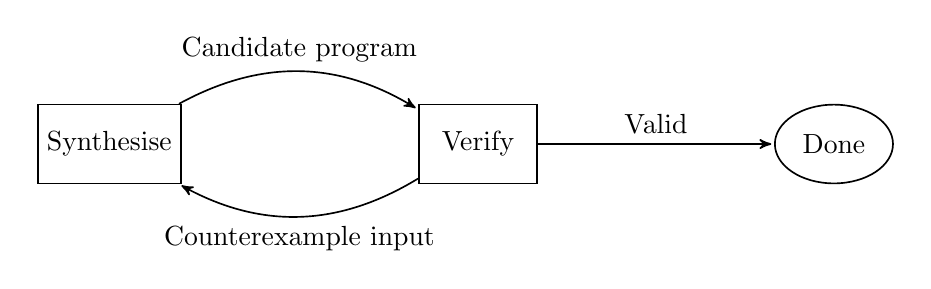
\begin{tikzpicture}[scale=0.5,->,>=stealth',shorten >=1pt,auto,
 semithick, initial text=]

  \matrix[nodes={draw, fill=none, scale=1, shape=rectangle, minimum height=1cm, minimum width=1.5cm},
          row sep=2cm, column sep=3cm] {
   \node (synth) {Synthesise};
   &
   \node (verif) {Verify}; %\\
   %\node[draw=none] {};
   &
   \node[ellipse] (done) {Done}; \\
  };

   \path
    (synth) edge [bend left] node {Candidate program} (verif)
    (verif) edge [bend left] node {Counterexample input} (synth)
    (verif) edge node {Valid} (done);
 \end{tikzpicture}
 
 \caption{Abstract synthesis refinement loop
 \label{fig:abstract-refinement}}
\end{figure*}



\begin{figure}
{\small
\begin{center}
\setlength{\tabcolsep}{16pt}
Integer arithmetic instructions:

\begin{tabular}{llll}
 \verb|add a b| & \verb|sub a b| & \verb|mul a b| & \verb|div a b| \\
 \verb|neg a| &   \verb|mod a b| & \verb|min a b| & \verb|max a b|
\end{tabular}

\medskip

Bitwise logical and shift instructions:

\begin{tabular}{lll}
 \verb|and  a b| & \verb|or   a b| & \verb|xor a b| \\
 \verb|lshr a b| & \verb|ashr a b| & \verb|not a|
\end{tabular}

\medskip

Unsigned and signed comparison instructions:

\begin{tabular}{lll}
 \verb|le  a b| & \verb|lt  a b| & \verb|sle  a b| \\
 \verb|slt a b| & \verb|eq  a b| & \verb|neq  a b|
\end{tabular}

Miscellaneous logical instructions:

\begin{tabular}{lll}
 \verb|implies a b| & \verb|ite a b c| & 
\end{tabular}

Floating point arithmetic:

\begin{tabular}{llll}
 \verb|fadd a b| & \verb|fsub a b| & \verb|fmul a b| & \verb|fdiv a b| 
\end{tabular}


\end{center}
}
 \caption{The language $\mathcal{L}$}
 \label{fig:l-language}
\end{figure}


\subsection{The Synthesis Algorithm}
As safety of a \newC program is efficiently 
%the quantifier free first-order fragment of the logic is efficiently 
decidable and a termination proof is expressible as a ground term of the \newC logic, we use
Counterexample Guided Inductive Synthesis (CEGIS)~\cite{lezama-thesis,sketch} to
check the validity of the synthesis formula. 
The core of the CEGIS algorithm is the refinement loop shown in Fig.~\ref{fig:abstract-refinement} and
detailed in Algorithm~\ref{fig:abstract-refinement-code}.  
The algorithm is divided into two
procedures: {\sc synth} (see Figure~\ref{fig:synth-dfd}) and {\sc verif}, which interact via
a finite set of test vectors {\sc inputs}, which is initialised to $\emptyset$.

The {\sc synth} procedure tries to find existential witnesses $(P, x_0)$ which satisfy the partial specification:
\[
 \exists P, x_0 . \forall x \in \text{\sc inputs} . \sigma(P, x_0, x)
\]

If {\sc synth} succeeds in finding a witness $(P, x_0)$, this witness is a candidate solution to the full
synthesis formula.  We pass this candidate solution to {\sc verif} which determines whether the candidate
does satisfy the specification on all inputs by checking satisfiability of the verification formula:
\[
 \exists x . \lnot \sigma(P, x_0, x)
\]

If this formula is unsatisfiable, the candidate solution is in fact a solution to the synthesis formula
and so the algorithm terminates.  Otherwise, the witness $x$ is an input on which the candidate solution fails
to meet the specification.  This witness $x$ is added to the {\sc inputs} set and the loop iterates again.

Concretely, {\sc synth} is implemented as shown in Figure~\ref{fig:synth-dfd}.  We start by taking the termination
specification and generating a C program which takes as input a candidate $(P, x_0)$ and asserts that the candidate
fails to meet the specification on at least on of the elements of {\sc inputs}.  So this program is unsafe iff there
is some candidate $(P, x_0)$ satisfying the specification for all the elements of {\sc inputs}.  Finding a new
candidate solution is therefore reduced to model checking this C program, which by construction is loop free.
The model checking is done using a combination of bounded model checking, explicit state enumeration and
genetic programming (GP).  The latter two techniques involve combining the previously generated C program,
along with code that searches for candidate solutions.  As well as efficiency, this has the side effect of
guaranteeing that we are verifying the exact semantics of the program under analysis as understood by a
compiler, rather than some ad-hoc abstraction of its semantics.  Finally, if any of the model checkers
finds a candidate solution it returns it.  The form of this candidate solution is yet another program,
this time written in the proof language $\mathcal{L}$.

Similarly, the {\sc verif} procedure is implemented by creating a C program that is unsafe iff
some input exists on which the candidate solution fails to meet the specification.  Again, symbolic
and explicit state model checking are used to decide the satisfiability of the verification formula.


%If the input set is finite, this procedure is guaranteed to terminate.



%% In some cases, it is faster to use an explicit-state model checker rather than a Bounded Model Checker.  
%% This is particularly true for the {\sc verif} component, 
%% where we have observed that incorrect programs tend
%% to be incorrect on a large fraction of the input space.  Counterexamples
%% are then very easy to find by explicit enumeration of a few inputs.
%% Since \newC is a fragment of C, we can generate an explicit-state
%% model checker using the same source files that we pass to {\sc cbmc}
%% and adding a small function to enumerate possible inputs.



%% ---  We begin with the program under analysis (the PUA).  From this we produce a specification (in second order logic)
%% encoding the termination of the PUA.  From the logical specification, we produce a program SYNTH.
%% SYNTH takes as input a proof and asserts that the proof is incorrect on at least one of the inputs being tracked so far.
%% Therefore, SYNTH is unsafe iff there is some proof that is correct for all of the tracked inputs.  Now we use testing
%% techniques to try to find a proof that causes SYNTH to crash.  The testing techniques we use are: model checking,
%% exhaustive search and genetic programming.  For the latter 2 techniques, we combine SYNTH with another program
%% (GP or EXPLICIT respectively) to create a program that searches for test vectors (proofs) that cause SYNTH
%% to crash.


%% In the {\sc synth} component, in order to find a candidate proof $P$ satisfying
%% $\sigma(i_1, P(i_1)) \land \ldots \land \sigma(i_N, P(i_N))$
%% for the tracked inputs $(i_1, \ldots, i_N)$, 
%% we attempt a safety proof.
%In order to determine the validity of the {\sc synth} formula, we can
%check the {\sc synth} program for safety.  


\begin{figure*}
\begin{center}
\tikzstyle{file}=[draw, text width=7.0em, text centered,
  minimum height=1.5em]
\tikzstyle{process} = [draw, minimum height=3em, circle]
\tikzstyle{line} = [draw, color=black, -latex']

\def\Divide#1#2{%
 \coordinate(a) at ($(#1.east) !.5! (#2.west)$);
 \coordinate(b) at (a |- 0,-3);
 \draw[dotted] (b) -- ++(0, 4.5);
}

\resizebox{\linewidth}{!}{
\begin{tikzpicture}[font=\sffamily]

\node [file] (pua) {input.c};

\path (pua.east)+(2,0) node [file] (spec) {\sc Termination Specification};
\path (spec.south)+(0.0, -1) node [file] (inputs) {\sc Tracked Inputs};
%% \path (synth.south)+(0.0, -0.5) node [file] (tests) {\sc tests.c};
%% \path (tests.south)+(0.0, -0.5) node [file] (interpreter) {\sc interpreter.c};
%% \path (interpreter.south)+(0.0, -0.5) node [file] (spec) {\sc spec.c};

%% \path (spec.east)+(2.0, -0.25) node [process] (merged) {merge};
\path (spec.east)+(2.0, -0.75) node [file] (file) {synth.c};

\path (file.east)+(2.0, 1.5) node [process] (cbmc) {\sc cbmc};
\path (file.east)+(2.0, 0.0) node [process] (gcc) {\sc Search};
\path (file.east)+(2.0, -1.5) node [process] (gp) {\sc GP};

\path (gcc.east)+(2.5, 0.0) node [file] (out) {Candidate Proof};

%\path [line] (spec) -- (merged);

\path [line] (pua) -- (spec);

\path [line] (spec) -- (file);
\path [line] (inputs) -- (file);

\path [line] (file) -- (cbmc);
\path [line] (file) -- (gcc);
\path [line] (file) -- (gp);


\path [line] (cbmc) -- (out);
\path [line] (gcc) -- (out);
\path [line] (gp) -- (out);

\Divide{pua}{spec}{puaspec}
%\Divide{spec}{file}{specfile}
\Divide{file}{gcc}{filegcc}
\Divide{gcc}{out}{gccout}

\draw (pua |- 0,-3) node [align=center] {Input program \\ (written in C)};

\coordinate (midspec) at ($(spec) !.5! (file)$);
\draw (midspec |- 0,-3) node [align=center] {Automatically generated specification \\ (written in C)};
%\draw (file |- 0,-3) node {Spec};
\draw (gcc |- 0,-3) node [align=center] {Model checker};
\draw (out |- 0,-3) node [align=center] {Proof \\ (written in $\mathcal{L}$)};

\end{tikzpicture}
}
\end{center}

\caption{Schematic diagram of {\sc synth}}
\label{fig:synth-dfd}
\end{figure*}


\subsection{Parameterising the Program Space}


In order to search the space of candidate programs, we parametrise
the language~$\mathcal{L}$ by program length, word width and number of constants,
inducing a lattice of progressively
more expressive languages.  We start by attempting to synthesise
a program at the lowest point on this lattice and increase the
parameters of~$\mathcal{L}$ until we reach a point at which
the synthesis succeeds.

As well as giving us an automatic search procedure, this parametrisation
greatly increases the efficiency of our system since languages
low down the lattice are very easy to decide safety for.  If a program
can be synthesised in a low-complexity language, the whole procedure
finishes much faster than if synthesis had been attempted in a
high-complexity language.


%% We introduce a novel parametrisation of the programming language
%% used to express our synthesised programs.
%% This parametrisation allows us to efficiently explore the program space
%% without relying on human guidance and also ensures that our programs
%% are of minimal length.

%% Our tool is the first we are aware of that is able to effectively
%% synthesise floating-point programs. We demonstrate this by
%% synthesising {\sc Fast2Sum} using Knuth's {\sc 2Sum}~\cite{taocp2} as
%% a specification.

%% ---Our exploration of the program space ensures that our programs are minimal in size.
%% --- We parametrise the space of programs in such a way that it can be explored automatically, rather than asking a human for hints.


%% We consider the following parameters:
%% \begin{itemize}
%% \item{Program Length: $l$}
%% The first parameter we introduce is program length, denoted by $l$.
%% At each iteration we synthesise programs of length exactly $l$.
%% We start with $l = 1$ and increment $l$ whenever we determine
%% that no program of length $l$ can satisfy the specification.  When we do
%% successfully synthesise a program, we are \emph{guaranteed that it
%% is of minimal length} since we have previously established that no
%% shorter program is correct.
%\item{Word Width: $w$}
%% An $\mathcal{L}$-program runs on a virtual machine (the $\mathcal{L}$-machine) that
%% has its own set of parameters.  The only relevant parameter is
%% the \emph{word width} of the $\mathcal{L}$-machine, that is, the number of bits
%% in each internal register and immediate constant.  This parameter is denoted by
%% $w$.  The size of the final SAT problem generated by {\sc cbmc} scales
%% polynomially with $w$, since each intermediate C variable corresponds
%% to $w$ propositional variables.


%\item{Number of Constants: $c$}
%% Instructions in $\mathcal{L}$ take either one or two operands.
%% Since any instruction whose operands are all constants can always be
%% eliminated (since its result is a constant), we know that a loop-free program
%% of minimal length will not contain any instructions with two constant
%% operands.  Therefore the number of constants that can appear in
%% a minimal program of length $l$ is at most $l$.  By minimising the number
%% of constants appearing in a program, we are able to use a particularly
%% efficient program encoding that speeds up the synthesis procedure
%% substantially.  The number of constants used in a program is the parameter $c$.

%\end{itemize}
%\subsubsection{Searching the Program Space}

The key to our automation approach is to come up with a sensible way in which to
adjust the $\mathcal{L}$-parameters in order to cover all possible programs.
After each round of {\sc synth}, we may need to adjust the parameters.  
%The
%logic for these adjustments is shown as a tree in Fig.~\ref{fig:paramsflow}.
Whenever {\sc synth} fails, we consider which parameter might have caused the
failure.  
%% There are two possibilities: either the program length $l$ was too small,
%% or the number of allowed constants $c$ was.  If $c < l$, we just increment $c$ and
%% try another round of synthesis, but allowing ourselves an extra program constant.
%% If $c = l$, there is no point in increasing $c$ any further.  This is because
%% no minimal $\mathcal{L}$-program has $c > l$, for if it did there would
%% have to be at least one instruction with two constant operands.  This
%% instruction could be removed (at the expense of adding its result as
%% a constant), contradicting the assumed minimality of the program.  So
%% if $c = l$, we set $c$ to 0 and increment $l$, before attempting
%% synthesis again.

%% If {\sc synth} succeeds but {\sc verif} fails, we have a candidate
%% program that is correct for some inputs but incorrect on at least
%% one input.  However, it may be the case that the candidate program
%% is correct for \emph{all} inputs when run on an $\mathcal{L}$-machine
%% with a small word size.  For example, we may have synthesised a
%% program which is correct for all 8-bit inputs, but incorrect for
%% some 32-bit input.  If this is the case (which we can determine
%% by running the candidate program through {\sc verif} using the smaller
%% word size), we may be able to produce a correct program for
%% the full $\mathcal{L}$-machine by using the constant extension rules
%% shown in Fig.~\ref{fig:generalize}.  If constant generalization
%% is able to find a correct program, we are done.  Otherwise,
%% we need to increase the word width of the $\mathcal{L}$-machine
%% we are currently synthesising for.


%% \section{Conclusion}

%% By expressing the program synthesis problem as a safety property for a
%% program interpreter, we have been able to harness the power of
%% state-of-the-art program analysis tools and reuse them in a new problem
%% domain.  We have implemented our algorithm as a freely downloadable tool
%% whose performance compares favourably to a recent program synthesiser. 
%% Finally, we have taken advantage of the expressiveness of our specification
%% language to make an initial step towards practical synthesis of
%% floating-point programs.




\section{Genetic Programming and Incremental Evolution}

We begin by observing that the asymptotic complexity of all of our synthesis
backends are equal, assuming $P \neq NP$.  This complexity is:

$$O\left(2^{K(f)}\right)$$

Where $K(f)$ is the Kolmogorov complexity of $f$, which is $O(\log Y^X) = O(X)$
so the complexity is doubly exponential in the width of $X$.

\begin{definition}
 A \emph{fitness landscape} is the space of all programs along with their fitness.
\end{definition}

\begin{theorem}
 Fitness landscapes form a lattice.  Adding test vectors corresponds to abstraction refinement on this
 lattice, which is why incremental GP works well.
\end{theorem}

\begin{proof}
 Trivial.
\end{proof}


\begin{conjecture}
 A single fitness landscape isn't really very smooth (e.g. small changes in program representation
 don't correspond to small changes in fitness), so GP probably shouldn't work very well.

 But it does.
\end{conjecture}


\section{Soundness, Completeness and Complexity}
\begin{theorem}
 {\sc Headshot} is sound -- if it says a program terminates then it does.
\end{theorem}

\begin{theorem}
 {\sc Headshot} is complete -- if a program terminates, {\sc Headshot} will find a proof that it does.
\end{theorem}

\begin{theorem}
 {\sc Headshot} is a decision procedure -- it always terminates.
\end{theorem}

\begin{theorem}
 {\sc Kalashnikov} has time complexity $NP^{NP}(K(\sigma))$
\end{theorem}

\begin{theorem}
 {\sc Headshot} uses a single call to {\sc Kalashnikov} and uses an encoding with $O(1)$
 overhead.  It therefore has time complexity $NP^{NP}(K(\tau(P))$ where $\tau(P)$ is the
 termination specification for program $P$.
\end{theorem}




In Section~\ref{sec:synthesis} we will describe a procedure for solving the synthesis formula.
This procedure has the property that it will find the shortest program meeting the
specification, and as a consequence the runtime of the program synthesiser is dominated
by the size of this shortest program.  To frame the discussion of the runtime of our
termination proving procedure, we first recall the definition of the Kolmogorov complexity
of a function $f$:

\begin{definition}[Kolmogorov complexity]
 The Kolmogorov complexity $K(f)$ is the length of the shortest program that
 computes $f$.
\end{definition}

We can extend this definition slightly to talk about the Kolmogorov complexity of a
synthesis problem in terms of its specification:

\begin{definition}[Kolmogorov complexity of a synthesis problem]
 The Kolmogorov complexity of a program specification $K(\sigma)$ is the length of the shortest
 program $P$ such that $P \models \sigma$.
\end{definition}

We will later show that the time complexity of our synthesis procedure is $NP^{NP}(K(\sigma))$,
which means that for even moderately large $K(\sigma)$ our procedure is intractably slow.  Conversely
if $K(\sigma)$ is small we will be able to find a termination proof, regardless of other parameters
such as the size of the program under analysis.  To put this another way, under the assumption
that $K(\sigma)$ is small for a program's termination problem, we will find a ranking function
quite rapidly.  We will now investigate the properties of functions with low Kolmogorov complexity,
and show that the assumption of a low-Kolmogorov ranking function is much weaker than the assumption
of a linear ranking function.


\begin{theorem}
 Linear functions have low Kolmogorov complexity.
\end{theorem}

\begin{proof}
 The function $f: X \to Y$ can be computed with a program consisting of
 $2 \cdot \dim(X) \cdot \dim(Y) - \dim(Y)$ instructions (1 multiplication and 1 addition for
 each cell in the matrix representing $f$).  Therefore,
 $K(f) \leq 2 \cdot \dim(X) \cdot \dim(Y) - \dim(Y)$.
\end{proof}

\begin{theorem}
Assuming a reasonable program encoding, the probability that a random program of length $l$ computes
a linear function is $O(2^{-l})$.
\end{theorem}

\begin{proof}
 (Do this proof properly).
 
 Otherwise, we'd need to have an exponential number of programs computing the same function.
 That would be an unreasonable program encoding.
\end{proof}


Therefore the number of non-linear functions $f$ with $K(f) \leq \kappa$
grows exponentially with $\kappa$, while the number of linear functions
grows only linearly.  This shows that assuming the existence of a linear
ranking function is much stronger than assuming the existence of a short
termination proof.  In addition to being a much weaker assumption,
we argue that low Kolmogorov complexity is a more natural assumption than
linearity.  Humans tend to write programs they can understand.  It's hard
to quantify exactly what ``understandable'' means, but we think that
``having a short proof'' is closer to the mark than ``having a linear proof''.



\iffalse
\begin{corollary}
 LKC is a weaker assumption than linearity.
\end{corollary}


\begin{theorem}
 LKC programs do not always have LKC ranking functions.
\end{theorem}

\begin{proof}
 This would solve the halting problem, Goldbach conjecture, Collatz conjecture.
\end{proof}

\begin{conjecture}
 High-Kolmogorov-complexity (HKC) programs often have LKC ranking functions.
\end{conjecture}

\begin{theorem}
 \textsc{Headshot} is biased towards finding ranking functions with
 low-Kolmogorov-complexity (LKC).
\end{theorem}

\begin{proof}
 Trivial.
\end{proof}

\subsection{The linearity assumption vs. the LKC one for ranking functions}

\begin{conjecture}
 Most LKC programs compute non-linear functions, but linear functions are LKC.
 So LKC is a weaker assumption than linearity.
\end{conjecture}

\begin{corollary}
 \textsc{Headshot} can often prove termination where linear methods cannot.
\end{corollary}
\fi


\section{Experiments}

We proved termination for a bunch of programs, see Fig.~\ref{fig:linear} and Fig.~\ref{fig:nonlinear}.

\begin{figure*}
\centering
\begin{tabular}{|l|r|r||r|r|r|r|}
\hline
    & LOC & \shortstack{Rank function \\ size} & \textsc{T2} & \textsc{ARMC} & \textsc{Headshot} & \textsc{Headshot-Linear} \\
    \hline
    \hline
 P1 & 10 & 3 & 100s & 70s & 0.1s & \bf{0.01s} \\
 P2 & 10 & 3 & 100s & 70s & 0.1s & \bf{0.01s} \\
 P3 & 10 & 3 & 100s & 70s & 0.1s & \bf{0.01s} \\
 \hline
\end{tabular}
\caption{Termination for linear programs with disjunctive, linear ranking functions\label{fig:linear}}
\end{figure*}

\begin{figure*}
\centering
\small
\begin{tabular}{|l|r|c|c|c|c|c|r|r|c|r|r|}
\hline
    & LOC & Terminates? & \shortstack{Linear \\ program?} & \shortstack{Linear ranking \\ function?}  & Conditional? & Float? & Dimension & \shortstack{Ranking \\ program size} & Res & Time (s) & Iterations\\
    \hline
    \hline




















svcomp1 & 17 & unk & true & true & false & false & 1 & 5 & term & 9.6s\\ 

svcomp2 & 13 & unk & false & true & false & false & 1 & 5 & term & 10.2s\\ 

svcomp3 & 15 & unk & true & true & false & false & unk & 5 & unk & T/O\\ 

svcomp4 & 14 & unk & true & unk & true & false & unk & 5 & unk & T/O\\ 



svcomp7 & 9 & unk & true & true & true & false & 1 & 5 & unk & T/O\\ 

svcomp8 & 9 & unk & true & unk & false & false & unk & 5 & unk & T/O\\ 

svcomp9 & 12 & unk & true & unk & false & false & unk & 5 & term & 9.3s\\ 

svcomp10 & 15 & unk & true & true & false & false & 1 & 5 & term & 61.2s\\ 

svcomp11 & 16 & unk & true & true & false & false & 1 & 5 & unk & T/O\\ 






svcomp17 & 17 & unk & true & true & false & false & 1 & 5 & nonterm & 19.0s\\ 








svcomp25 & 12 & unk & true & true & false & false & 1 & 5 & unk & T/O\\ 

svcomp26 & 23 & unk & true & true & false & false & 1 & 5 & term & 38.7s\\ 

svcomp27 & 13 & unk & true & true & false & false & 1 & 5 & unk & T/O\\ 

svcomp28 & 18 & unk & true & true & false & false & 1 & 5 & unk & T/O\\ 

svcomp29 & 9 & unk & true & true & false & false & 1 & 5 & unk & T/O\\ 








svcomp37 & 22 & unk & true & true & false & false & 1 & 5 & term & 12.3s\\ 

svcomp38 & 16 & unk & true & true & false & false & 1 & 5 & unk & T/O\\ 

svcomp39 & 56 & unk & true & true & false & false & 1 & 5 & unk & T/O\\ 



svcomp42 & 22 & unk & true & true & false & false & 1 & 5 & unk & T/O\\ 



    \hline
\end{tabular}

\caption{\textsc{Headshot} termination for nonlinear programs with nonlinear ranking functions\label{fig:nonlinear}}
 \end{figure*}


\bibliographystyle{abbrvnat}
\bibliography{synth}{}

\end{document}
